\documentclass[addpoints,12pt]{exam}
\usepackage[spanish]{babel}
%\usepackage[latin1]{inputenc}
\usepackage[utf8x]{inputenc}
\usepackage{graphicx}
\pagestyle{empty}
\begin{document}
\begin{center}
\fbox{\fbox{\parbox{5.5in}{\centering {\LARGE EXAMEN TIPO B}\\El ejercicio se realizará en eclipse. Usa un workspace distinto al que usas de forma habitual. Crea un proyecto de java nuevo denominado Examen donde desarrollar las carpetas, packages y programas}}}
\end{center}
\vspace{0.1in}
La estructura del proyecto será la siguiente:
\begin{itemize}
\item Un proyecto denominado \emph{Examen}
\item Dos carpetas en la raiz del proyecto denominadas \emph{database} y \emph{lib}. En la primera debe situar la base de datos \emph{company.db} y en la otra se coloca el driver de \emph{sqlite}. Se debe añadir a las bibliotecas del proyecto, de manera que la importación del mismo no requiera volver añadir este \emph{jar}
\item Un package denominado \emph{clases} donde colocar las disitintas clases y otro package denominado \emph{test} donde colocar el programa que arranca la aplicación.
\end{itemize}
La aplicación usará como persistencia la base de datos antes mencionada, con el siguiente diagram ER.\\
%\makebox[\textwidth]{Nombre:\enspace\hrulefill}
\begin{figure}[h]
\begin{center}
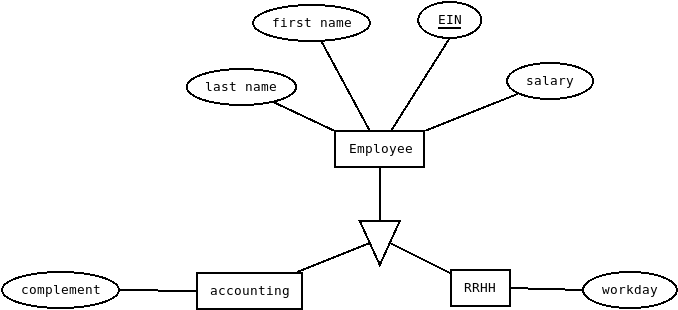
\includegraphics[scale=0.5]{er.png}
%
\end{center}
\end{figure}
\\
Dicha base de datos hace referencia a la estructura jeráquica de una empresa, con dos departamentos, contabilidad y recursos humanos.\\
Los empleados quedan determinados por el nombre y apellidos, mas un identificador único (\emph{EIN})  y su salario base.\\
En el departamento de contabilidad, cada empleado tiene un complemento adicional a su sueldo.\\
Y en el caso del departamento de recursos humanos (\emph{RRHH}) se indica las horas de su jornada laboral (\emph{workday})
\newpage
\begin{questions}
\question Queremos realizar un aplicación que realice algunas operaciones de tipo \emph{CRUD} sobre dicha base de datos, para esto se debe realizar la estructura de clases de acuerdo con el paradigma de herencia de \emph{POO} que ofrece \emph{Java}. Para esto se implementará una clase para cada entidad. Los atributos de cada clase deberán estar acordes -en nombre y tipo- con las columnas de cada tabla, para esto es aconsejable mirar el diagrama ER y el esquema de cada tabla en la base de datos. En relación a las clases se tendrán en cuenta:
\begin{description}
\item[clase Employee] que hace referencia al departamento de contablidad. {\small \textbf{NO}} sobrescribe el método \emph{toString()}
\item[clase Accounting] sobreescribe el método \emph{toString()} para que muestre con el método \emph{format} de la clase \emph{String} los datos referentes a:
\begin{itemize}
\item First name
\item Las Name
\item EIN (identificador de trabajador);
\item Sueldo total que incluye el salario del empleado mas el complemento por trabajar en este departamento de contabilidad.
\end{itemize}
\item[clase RRHH] que hace referencia al departamento de recursos humanos. Esta clase sobreescribe el método \emph{toString()} para mostrar todos los campos de la clase padre y de esta propia clase. También usaremos el método \emph{format} de la clase \emph{String}
\end{description}
Se creará la siguiente interfaz:
\begin{figure}[h]
\begin{center}
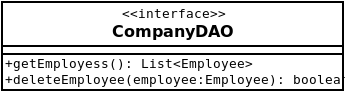
\includegraphics[scale=0.7]{dao1.png}
\end{center}
\end{figure}
Además se crearán las siguientes clases:
\begin{description}
\item[Clase ConnectionDB] que mediante patrón \emph{singleton} se encargue de abrir y cerrar la conexión a la BD. Además debemos tener en cuenta que la base de datos relacional implica la integridad referencial, por lo que debemos incluirlo en la configuración de la conexión:
\begin{verbatim}
SQLiteConfig config = new SQLiteConfig () ;
config.enforceForeignKeys ( true ) ;
DriverManager.getConnection ( nombreBD , config.toProperties () );
\end{verbatim}
\item[Clase EmployeeDAOImplentation] que se encarga de la implementación de la interfaz antrior.
\newpage
\item[Clase App] que arranca la aplicación, muestra un menú donde nos de a elegir  lo siguiente:
\begin{itemize}
\item Mostrar los empleados del departamento de contabilidad.
\item Mostrar los empleados del departamento de recursos humanos.
\item Borrar un empleado, para esto se solicitará  un \emph{EIN} válido para realizar el borrado. La validación se hará en la interfaz en un método estático. Un \emph{EIN} válido tiene el formato \emph{dd-ddddddddd} Donde \emph{d} es un dígito entre 0 y 9.
\end{itemize}
\end{description}


Criterios de evaluación:
\begin{description}
\item[0.5 ptos] Por la correcta implementación de la estructura del proyecto.
\item[0.5 ptos.] Por la clase \emph{ConnectionDB}
\item[2 ptos.] Por las clases que implementan la estructura de herencia.
\item[1 pto.] Por la interfaz, incluyendo el método de validación del \emph{EIN}
\item[3 ptos.] Por la clase que implementa la interfaz
\item[3 ptos.] Por la clase \emph{Appn}
\end{description}
\textbf{Formato del fichero de subida:} se subirá el \emph{workspace} completo del proyecto del examen.
\end{questions}
\end{document}
